%% LyX 2.4.2.1 created this file.  For more info, see https://www.lyx.org/.
%% Do not edit unless you really know what you are doing.
\documentclass[10pt,oneside,english,no-math]{book}
\usepackage{amsmath}
\usepackage{amsthm}
\usepackage{amssymb}
\usepackage{fontspec}
\renewcommand{\familydefault}{\sfdefault}
\setcounter{secnumdepth}{3}
\setcounter{tocdepth}{3}
\setlength{\parindent}{0bp}
\usepackage{color}
\usepackage{array}
\usepackage{float}
\usepackage{mathtools}
\usepackage{multirow}
\usepackage{algorithm2e}
\usepackage{varwidth}
\usepackage{dsfont}
\usepackage{graphicx}
\usepackage{geometry}
\geometry{verbose,tmargin=2cm,bmargin=2cm,lmargin=2cm,rmargin=2cm,headheight=0cm,headsep=1cm,footskip=1cm}
\usepackage{setspace}
\onehalfspacing
\usepackage[pdfusetitle,
 bookmarks=true,bookmarksnumbered=false,bookmarksopen=false,
 breaklinks=false,pdfborder={0 0 0},pdfborderstyle={},backref=false,colorlinks=true]
 {hyperref}
\hypersetup{
 linkcolor=blue, urlcolor=marineblue, citecolor=blue, pdfstartview={FitH}, hyperfootnotes=false, unicode=true}

\makeatletter

%%%%%%%%%%%%%%%%%%%%%%%%%%%%%% LyX specific LaTeX commands.
\providecommand\textquotedblplain{%
  \bgroup\addfontfeatures{RawFeature=-tlig}\char34\egroup}
%% Because html converters don't know tabularnewline
\providecommand{\tabularnewline}{\\}
%% Variable width box for table cells
\newenvironment{cellvarwidth}[1][t]
    {\begin{varwidth}[#1]{\linewidth}}
    {\@finalstrut\@arstrutbox\end{varwidth}}

%%%%%%%%%%%%%%%%%%%%%%%%%%%%%% Textclass specific LaTeX commands.
\newtheoremstyle{defuprightbrackets}%
  {3pt}{3pt}%
  {\upshape}%
  {}%
  {\bfseries}%
  {.}% no punctuation
  { }%
  {\thmname{#1}\thmnumber{ #2}\thmnote{ [\textbf{\itshape #3}]}}%
\theoremstyle{defuprightbrackets}
\theoremstyle{definition}
    \ifx\thechapter\undefined
      \newtheorem{defn}{\protect\definitionname}
    \else
      \newtheorem{defn}{\protect\definitionname}[chapter]
    \fi
\theoremstyle{defuprightbrackets}
\ifx\thechapter\undefined
  \newtheorem{thm}{\protect\theoremname}
\else
  \newtheorem{thm}{\protect\theoremname}[chapter]
\fi
% Do nothing special here
\theoremstyle{defuprightbrackets}
\ifx\thechapter\undefined
  \newtheorem{claim}{\protect\claimname}
\else
  \newtheorem{claim}{\protect\claimname}[chapter]
\fi
\theoremstyle{defuprightbrackets}
\ifx\thechapter\undefined
  \newtheorem{cor}{\protect\corname}
\else
  \newtheorem{cor}{\protect\corname}[chapter]
\fi
\theoremstyle{defuprightbrackets}
\ifx\thechapter\undefined
  \newtheorem{rem}{\protect\remname}
\else
  \newtheorem{rem}{\protect\remname}[chapter]
\fi
\theoremstyle{defuprightbrackets}
\ifx\thechapter\undefined
  \newtheorem{alg}{\protect\algorithmname}
\else
  \newtheorem{alg}{\protect\algorithmname}[chapter]
\fi
\theoremstyle{defuprightbrackets}
\ifx\thechapter\undefined
  \newtheorem{prob}{\protect\problemname}
\else
  \newtheorem{prob}{\protect\problemname}[chapter]
\fi
\theoremstyle{defuprightbrackets}
\ifx\thechapter\undefined
  \newtheorem{conc}{\protect\conclusionname}
\else
  \newtheorem{conc}{\protect\conclusionname}[chapter]
\fi

\@ifundefined{date}{}{\date{}}
%%%%%%%%%%%%%%%%%%%%%%%%%%%%%% User specified LaTeX commands.
% --- Load amsthm package for theorem styles ---
\usepackage{amsthm}

\usepackage[most]{tcolorbox}


% --- Shared theoremstyle (one place only!) ---
\newtheoremstyle{defuprightbrackets}%
  {3pt}{3pt}% space above/below
  {\upshape}% body font
  {}% indent amount
  {\bfseries}% head font
  {}
  { }% space after theorem head
  {\thmname{#1}\thmnumber{ #2}\thmnote{ [\textbf{#3}]}}%

% --- Apply this style to all environments ---
\theoremstyle{defuprightbrackets}

% --- Define all environments to use LyX's language macros ---
\ifx\thechapter\undefined
  \newtheorem{mytheorem}{\protect\theoremname}
\else
  \newtheorem{mytheorem}{\protect\theoremname}[chapter]
\fi

% --- All other environments share the 'mytheorem' counter ---
\newtheorem{mydefinition}[mytheorem]{\protect\definitionname}
\newtheorem{mylemma}[mytheorem]{\protect\lemmaname}
\newtheorem{myproposition}[mytheorem]{\protect\propositionname}
\newtheorem{mycorollary}[mytheorem]{\protect\corollaryname}
\newtheorem{myclaim}[mytheorem]{\protect\claimname}
\newtheorem{myconjecture}[mytheorem]{\protect\conjecturename}
\newtheorem{myremark}[mytheorem]{\protect\remarkname}
\newtheorem{myexample}[mytheorem]{\protect\examplename}
\newtheorem{myexercise}[mytheorem]{\protect\exercisename}
\newtheorem{myproblem}[mytheorem]{\protect\problemname}
\newtheorem{myfact}[mytheorem]{\protect\factname}
\newtheorem{mynotation}[mytheorem]{\protect\notationname}
\newtheorem{myassumption}[mytheorem]{\protect\assumptionname}
\newtheorem{mysummary}[mytheorem]{\protect\summaryname}
\newtheorem{myconclusion}[mytheorem]{\protect\conclusionname}
\newtheorem{myalgorithm}[mytheorem]{\protect\algorithmname}
\newtheorem{myaxiom}[mytheorem]{\protect\axiomname}
\newtheorem{mycondition}[mytheorem]{\protect\conditionname}
\newtheorem{myquestion}[mytheorem]{\protect\questionname}

% --- Unnumbered environments ---
\newtheorem*{mysolution}{\protect\solutionname}

% --- Optional: change QED symbol for proofs ---
\renewcommand{\qedsymbol}{$\square$}

% Allows fancy stuff in the page header
\usepackage{fancyhdr}
\pagestyle{fancy}

\usepackage{enumitem}
\setlist[itemize,1]{label={\fontfamily{cmr}\fontencoding{T1}\selectfont\textbullet}}

%Allows circuit drawing
\usepackage{circuitikz}

%Allows plotting graphs
\usepackage{pgfplots}

\usetikzlibrary{svg.path,decorations.pathmorphing, backgrounds,decorations.pathreplacing, automata, shapes.geometric, arrows.meta, positioning, calc}

% =========================================================
% GLOBAL TIKZ SETTINGS (For White/Print Backgrounds)
% =========================================================
\usepackage{tikz}
\usetikzlibrary{arrows.meta, positioning, calc, shapes.geometric}

\tikzset{
    % Standard 'person' nodes (Alice, Bob, Eve)
    person/.style={
        circle, 
        draw, 
        minimum size=1cm, 
        line width=1.5pt, 
        fill=white,           % Clean white fill for standard pages
        font=\bfseries
    },
    % Experiment Boxes (Challenger/Adversary)
    box/.style={
        draw, 
        thick, 
        rounded corners, 
        minimum width=2.5cm, 
        minimum height=1.5cm, 
        align=center,
    },
    % Challenger: Light blue tint from lecture
    chalbox/.style={
        box, 
        fill=blue!20, 
        draw=blue!50!black
    },
    % Adversary: Light red tint from lecture
    advbox/.style={
        box, 
        fill=red!20, 
        draw=red!50!black
    },
    % Default arrow style
    arrow/.style={
        ->, 
        >=Stealth, 
        thick,
        line width=1pt
    },
    % Distance between nodes
    node distance=1.5cm
}

\usepackage{mathtools}
\let\savedleft\left
  \let\savedright\right

  % Redefine \left and \right to insert the pairing-group hack
  \renewcommand{\left}{\mathopen{}\mathclose\bgroup\savedleft}
  \renewcommand{\right}{\aftergroup\egroup\savedright}

% Necessary Commands:
\usepackage{autobreak}
\usepackage[T1]{fontenc}
\usepackage{relsize}

% Convert the QED Symbol at the end of proofs to a solid black square (credit: Yakir Oz):
\usepackage{amssymb}
\renewcommand{\qedsymbol}{$\blacksquare$}


% Create disjoint union symbols:
\makeatletter
\def\moverlay{\mathpalette\mov@rlay}
\def\mov@rlay#1#2{\leavevmode\vtop{%
   \baselineskip\z@skip \lineskiplimit-\maxdimen
   \ialign{\hfil$\m@th#1##$\hfil\cr#2\crcr}}}
\newcommand{\charfusion}[3][\mathord]{
    #1{\ifx#1\mathop\vphantom{#2}\fi
        \mathpalette\mov@rlay{#2\cr#3}
      }
    \ifx#1\mathop\expandafter\displaylimits\fi}
\makeatother
\newcommand{\cupdot}{\charfusion[\mathbin]{\cup}{\cdot}}
\newcommand{\bigcupdot}{\charfusion[\mathop]{\bigcup}{\cdot}}


\newcommand{\kaliLargeLand}{\mathop{\mathlarger{\mathlarger{\mathlarger{\land}}}}}
\newcommand{\hebtext}[1]{\mbox{\R{\#1}}}


% Or if you have EB Garamond:
% \newfontfamily\erlangfont{EB Garamond}[Style=Italic]

% --- Redefine the 'proof' environment to match LyX style ---
% (Bold, Upright Label; Upright Body; UNIFORM 3pt spacing)
\makeatletter
\renewenvironment{proof}[1][\proofname]{\par
  \pushQED{\qed}%
  \normalfont \topsep3pt\relax  % <-- THIS IS THE SPACING FIX
  \trivlist
  \item[\hskip\labelsep
        \bfseries
    #1\@addpunct{.}]\ignorespaces
}{%
  \popQED\endtrivlist\@endpefalse
}
\makeatother

% Define colors for the dark theme
\definecolor{deepbg}{RGB}{22, 33, 62}       % Dark Navy Background
\definecolor{cyanpath}{RGB}{0, 255, 255}    % Bright Cyan for Gaussian paths
\definecolor{poissonorange}{RGB}{255, 165, 0} % Orange for Poisson steps
\definecolor{textwhite}{RGB}{240, 240, 240}

% =========================================================
% BOXED PROOF REDEFINITION (English Overriding)
% =========================================================
% 1. Define the English Proof Style
\tcbset{
  engproofstyle/.style={
    enhanced,
    breakable,
    width=\textwidth,
    colback=white,
    colframe=black!75, 
    colbacktitle=black!5!white, 
    coltitle=black, 
    fonttitle=\bfseries,
    % Anchored to top-left for English context
    attach boxed title to top left={yshift=-2mm, xshift=5mm}, 
    boxed title style={boxrule=0.4pt, colframe=black!75},
    separator sign none,
    after upper={\par\hfill\qedsymbol} % Auto-QED
  }
}

% 2. Override the standard 'proof' environment
\renewenvironment{proof}[1][Proof]{%
  \begin{tcolorbox}[engproofstyle, title=#1]
}{%
  \end{tcolorbox}
}

\makeatother

\usepackage{polyglossia}
\setdefaultlanguage[variant=american]{english}
\providecommand{\algorithmname}{Algorithm}
\providecommand{\claimname}{Claim}
\providecommand{\conclusionname}{Conclusion}
\providecommand{\corname}{Corollary}
\providecommand{\corollaryname}{Corollary}
\providecommand{\definitionname}{Definition}
\providecommand{\problemname}{Problem}
\providecommand{\proofname}{Proof}
\providecommand{\remname}{Remark}
\providecommand{\remarkname}{Remark}
\providecommand{\theoremname}{Theorem}

\begin{document}
\begin{titlepage}
    % This scope ensures the dark background covers the entire physical page
    \pagecolor{deepbg}\color{textwhite}
    \begin{tikzpicture}[remember picture, overlay]
      

        % === 3. YOUR PERSISTENT CENTER TEXT ===
        \node[anchor=center] at (current page.center) {
            \begin{minipage}{\textwidth}
                \centering
                {\sffamily\Huge \textbf{INTRODUCTION TO} \par}
                \vspace{0.4cm}
                {\sffamily\bfseries\fontsize{46}{52}\selectfont \textcolor{cyanpath}{MODERN} \textcolor{poissonorange}{CRYPTOGRAPHY} \par}
				\vspace{0.4cm}
 				\color{textwhite}
				{\sffamily\Large \textbf{0368-3049} \par}
				\vspace{0.3cm}
             
	
                \vspace{3.2cm} % Adjusted to sit between protocol lines
                {\sffamily\Large Based on lectures by \par}
                \vspace{0.3cm}
                {\sffamily\Large\bfseries Prof. Benny Applebaum \par }
				\vspace{0.3cm}
				{\sffamily\Large and recitations by \par}
                \vspace{0.3cm}
                {\sffamily\Large\bfseries  Tomer Solomon \par }
                
                \vspace{2.8cm}
                
                {\sffamily\huge \textbf{written by Ron Goldman} \par}
                \vspace{0.6cm}
 				{\sffamily\Large \textbf{2025-2026} \par}
            \end{minipage}
        };
    \end{tikzpicture}
\end{titlepage}
\nopagecolor\color{black}

\tableofcontents{}

\global\long\def\KK{\mathcal{K}}%
\global\long\def\MM{\mathcal{M}}%
\global\long\def\CC{\mathcal{C}}%
\global\long\def\enc{\mathsf{Enc}}%
\global\long\def\dec{\mathsf{Dec}}%
\global\long\def\ind#1#2{\approx_{#1,#2}}%
\global\long\def\r{\xleftarrow{\mathsf{R}}}%
\global\long\def\prg{\mathsf{PRG}}%
\global\long\def\binary{\left\{  0,1\right\}  }%
\global\long\def\str#1{\binary^{#1}}%
\global\long\def\P{\boldsymbol{\mathsf{P}}}%
\global\long\def\NP{\boldsymbol{\mathsf{NP}}}%
\global\long\def\prf{\mathsf{PRF}}%
\global\long\def\mac{\mathsf{MAC}}%
\global\long\def\tg{\mathsf{tag}}%
\global\long\def\TT{\mathcal{T}}%


\part{Private-key Cryptography}


\chapter{Introduction}

Let $\KK,\MM,\CC$ be finite sets.

\section{Notations and Definitions}
\begin{mydefinition}[Encryption]
 A function $\enc:\KK\times\MM\xrightarrow{}\CC$. For all $k\in\KK,m\in\MM$,
the message after the encryption, $c=\enc\left(k,m\right)\triangleq\enc_{k}\left(m\right)$,
is the \textbf{ciphertext}.
\end{mydefinition}
%
\begin{mydefinition}[Decryption]
 A function $\dec:\KK\times\CC\xrightarrow{}\MM$. For all $k\in\KK,c\in\CC$,
the message before the encryption, $m=\dec\left(k,c\right)\triangleq\dec_{k}\left(c\right)$,
is the \textbf{plaintext}. 
\end{mydefinition}
%
\begin{mydefinition}[Correctness]
 For all $m\in\MM$, $\dec_{k}\left(\enc_{k}\left(m\right)\right)=m$.
\end{mydefinition}

\subsection{Communication Model}

Let us welcome the three major players in this field, \textcolor{blue}{Alice},
\textcolor{blue}{Bob}, and \textcolor{red}{Eve} (claps!).

\begin{center}
\begin{tikzpicture}
    % Parties
    \node[person, color=blue] (A) at (0,0) {\textcolor{white}{\textbf{A}}};
    \node[person, color=blue, right=5cm of A] (B) {\textcolor{white}{\textbf{B}}};
    \node[person, color=red, dashed] (E) at (2.5,-1.5) {\textcolor{white}{\textbf{E}}};
    
    % Labels (Explicitly white for visibility)
    \node[below=0.2cm of A, color=blue, font=\sffamily\small] {Alice};
    \node[below=0.2cm of B, color=blue, font=\sffamily\small] {Bob};
    \node[below=0.2cm of E, color=red, font=\sffamily\small] {Eve};

    % Communication channel
    \draw[->, >=Stealth, line width=1.2pt] 
        (A.east) -- node[above, pos=0.5] {$c = \enc_k(m)$} (B.west);
    
    % Eavesdropping intercept
    \draw[->, >=Stealth, red, dashed, thick] (2.5,0) -- (E.north);

\end{tikzpicture}
\end{center}

In our model, the \textquotedbl major players\textquotedbl{} interact
as follows:
\begin{itemize}
\item \textbf{Parties:} Alice and Bob are the legitimate participants.
\item \textbf{Adversary:} Eve is the eavesdropper monitoring the line.
\item \textbf{Channel: }A reliable communication line exists between Alice
and Bob.
\item \textbf{The Shared Secret:} They utilize an encryption scheme $\left(\enc,\dec\right)$
that is \emph{known }to Eve, and a \emph{secret }key $k$.
\item \textbf{The Goal:} Alice wants to send a message $m$ to Bob such
that it remains \emph{confidential}.
\end{itemize}
%

\section{Perfect Secrecy}
\begin{mydefinition}
Two distributions $X,Y$ over $\mathcal{D}$ are \textbf{equal}, denoted
by $X\equiv Y$, if $\forall d\in\mathcal{D}.\ \Pr\left[X=d\right]=\Pr\left[Y=d\right]$.
\end{mydefinition}
%
\begin{mydefinition}[Perfect Secrecy (Shannon 1949)]
 We say $\left(\enc,\dec\right)$ is \textbf{perfectly secret }if
for any a priori distribution $M$ of messages, and $k\r\KK$, $M|\enc_{k}\left(M\right)\equiv M$.
\end{mydefinition}
%
\begin{mydefinition}[Perfect Indistinguishability]
We say $\left(\enc,\dec\right)$ is \textbf{perfectly} \textbf{indistinguishable}
if for any $m_{0},m_{1}\in\mathcal{M}$ of equal length, if $k\r\KK$,
then $\enc_{k}\left(m_{0}\right)\equiv\enc_{k}\left(m_{1}\right)$.
\end{mydefinition}
%
\begin{mydefinition}[Indistinguishability Game]
 For an \emph{adversary }$\mathcal{A}:\CC\xrightarrow{}\binary$
we define the following game:
\begin{itemize}
\item $\mathcal{A}$ chooses messages $m_{0},m_{1}\in\MM$.
\item We sample a key $k\r\KK$ and a bit $b\r\binary$.
\item We send $\enc_{k}\left(m_{b}\right)$ to $\mathcal{A}$, called the
\emph{challenge}.
\item $\mathcal{A}$ outputs a bit $b'$.
\end{itemize}
We say that $\mathcal{A}$ \textbf{wins} if $b'=b$, and we denote
$\Pr\left[\mathcal{A}\text{ wins}\right]\triangleq\Pr\left[b=b'\right]$.
\end{mydefinition}
\begin{thm}
Let $\left(\enc,\dec\right)$ be a symmetric encryption scheme. Then,
the following are equivalent:
\begin{enumerate}
\item $\left(\enc,\dec\right)$ is \emph{perfectly secret}.\label{enu:th1ps}
\item $\left(\enc,\dec\right)$ is \emph{perfectly indistinguishable}.\label{enu:th1pi}
\item For any adversary $\mathcal{A}$, $\Pr\left[\mathcal{A}\text{ wins}\right]=\frac{1}{2}$.\label{enu:th1ig}
\end{enumerate}
\begin{proof}
$(\ref{enu:th1ps})\iff(\ref{enu:th1pi})$ was left to HW1, Q1. $\underline{(\ref{enu:th1pi})\Longrightarrow(\ref{enu:th1ig}):}$
Let $\mathcal{A}$ be an adversary, WLOG deterministic, and let $m_{0},m_{1}\in\MM$.
Define $S_{b}\triangleq\mathcal{A}^{-1}\left(\left\{ b\right\} \right)$
for $b\in\binary$, then $S_{0}\uplus S_{1}=\CC$. Let $b'=\mathcal{A}\left(m_{b}\right)$,
where $b\xleftarrow{}\binary$, since $\left(\enc,\dec\right)$ is
p.i., then by total probability
\begin{align*}
\Pr\left[\mathcal{A}\text{ wins}\right] & =\Pr\left[b'=b|b=0\right]\Pr\left[b=0\right]+\Pr\left[b'=b|b=1\right]\Pr\left[b=1\right]\\
 & =\frac{1}{2}\left(\Pr\left[\enc_{k}\left(m_{0}\right)\in S_{0}\right]+\Pr\left[\enc_{k}\left(m_{1}\right)\in S_{1}\right]\right)\\
 & =\frac{1}{2}\left(\Pr\left[\enc_{k}\left(m_{0}\right)\in S_{0}\right]+\Pr\left[\enc_{k}\left(m_{0}\right)\in S_{1}\right]\right)\\
 & =\frac{1}{2}\Pr\left[\enc_{k}\left(m_{0}\right)\in S_{0}\uplus S_{1}\right]=\frac{1}{2}.
\end{align*}
 $\underline{(\ref{enu:th1ig})\Longrightarrow(\ref{enu:th1pi}):}$
Suppose $\left(\enc,\dec\right)$ is not p.i., then there must be
some $m_{0},m_{1}\in\MM,c^{*}\in\CC$ s.t.
\[
\alpha=\Pr\left[\enc_{k}\left(m_{0}\right)=c^{*}\right]>\Pr\left[\enc_{k}\left(m_{1}\right)=c^{*}\right]=\beta.
\]
Consider the adversary $\mathcal{A}$ that selects the messages $m_{0},m_{1}$,
and on input $c\in\CC$, $\mathcal{A}\left(c\right)=\mathds{1}\left[c\neq c^{*}\right]$.
Then by total probability
\begin{align*}
\Pr\left[\mathcal{A}\text{ wins}\right] & =\Pr\left[b'=b|b=0\right]\Pr\left[b=0\right]+\Pr\left[b'=b|b=1\right]\Pr\left[b=1\right]\\
 & =\frac{1}{2}\left(\Pr\left[\enc_{k}\left(m_{0}\right)=c^{*}\right]+\Pr\left[\enc_{k}\left(m_{1}\right)\neq c^{*}\right]\right)\\
 & =\frac{1}{2}\left(\alpha+\left(1-\beta\right)\right)=\frac{1}{2}+\frac{1}{2}\left(\alpha-\beta\right)>\frac{1}{2}.
\end{align*}
\end{proof}
\end{thm}

\section{One-Time Pad}
\begin{mydefinition}[One-Time Pad]
 Let $\MM=\KK=\CC=\str n$, then for any $m,k,c\in\str n$ (where
$\oplus$ is bitwise XOR), we define the \textbf{one-time pad }scheme:
\begin{align*}
\enc_{k}\left(m\right)=m\oplus k & , & \dec_{k}\left(c\right)=c\oplus k & .
\end{align*}
\end{mydefinition}
\begin{thm}
One-Time Pad is \emph{perfectly secret}.
\begin{proof}
It is suffice to show the following claim:
\begin{claim}
For any $m,c\in\str n$
\[
\Pr_{k\r\str n}\left[\enc_{k}\left(m\right)=c\right]=\frac{1}{2^{n}}\iff\enc_{k}\left(m\right)\sim\mathcal{U}_{n}
\]
\end{claim}
The claim implies the theorem from transitivity, for any $m_{0},m_{1}\in\str n$,
where $k\r\str n$:
\[
\enc_{k}\left(m_{0}\right)\equiv\mathcal{U}_{n}\equiv\enc_{k}\left(m_{1}\right)
\]

\textbf{Proof of the claim.} Let $m,c\in\str n$, then:
\[
\Pr_{k}\left[\enc_{k}\left(m\right)=c\right]=\Pr_{k}\left[m\oplus k=c\right]=\Pr_{k}\left[k=m\oplus c\right]=\frac{1}{2^{n}}
\]
 since $m\oplus c$ is a constant and $k\sim\mathcal{U}_{n}$.
\end{proof}
\end{thm}

\section{Shannon's Theorem}
\begin{thm}[Shannon]
 If $\left(\enc,\dec\right)$ is perfectly secret, then $\left|\KK\right|\geq\left|\MM\right|$.
\begin{proof}
Define a two-sided graph $G=\left(V,E\right)$ where $V=\MM\uplus\CC$,
$\left\{ m,c\right\} \in E$ if and only if there exists $k\in\KK$
s.t. $\enc_{k}\left(m\right)=c$. Assume for sake of contradiction
that $\left|\KK\right|<\left|\MM\right|$, and let $\left\{ m,c\right\} \in E$.
\begin{claim}
$c$ is connected to at most $\left|\KK\right|$ messages, i.e. $\deg\left(c\right)\leq\left|\KK\right|$.
\end{claim}
\textbf{Proof of the claim.} Assume for sake of contradiction that
$\deg\left(c\right)>\left|\KK\right|$. By the pidgeonhole principle,
there exists a key $k\in\KK$ and two messages $m_{0},m_{1}\in\MM$
s.t. $c=\enc_{k}\left(m_{0}\right)=\enc_{k}\left(m_{1}\right)$ and
that is a contradiction to the correctness of $\left(\enc,\dec\right)$.
\begin{cor}
There exists a message $m^{*}\in\MM$ that isn't a neighbor of $c$.
\end{cor}
For any key $k\in\KK$, it holds that $\enc_{k}\left(m^{*}\right)\neq c$,
and thus ${\displaystyle \Pr_{k}\left[\enc_{k}\left(m^{*}\right)=c\right]=0}$.

Since $\left\{ m,c\right\} \in E$, there exists a key $k'\in\KK$
s.t. $\enc_{k'}\left(m\right)=c$, and thus ${\displaystyle \Pr_{k}\left[\enc_{k}\left(m\right)=c\right]\geq\frac{1}{\left|\KK\right|}}>0$.

We then conclude $\enc_{k}\left(m^{*}\right)\not\equiv\enc_{k}\left(m\right)$,
where $k\xleftarrow{}\KK$, which is a contradiction.
\end{proof}
\end{thm}


\chapter{Computational Secrecy \& Pseudorandomness}


\section{Computational Secrecy}
\begin{claim}[Perfect Secrecy Revisited]
 $\left(\enc,\dec\right)$ has perfect secrecy if and only if for
any $m_{0},m_{1}\in\MM$ of equal length, if we denote $c_{0}=\enc_{k}\left(m_{0}\right),c_{1}=\enc_{k}\left(m_{1}\right)$
for all $k\in\KK$, then for any adversary $\mathcal{A}$, 
\[
{\displaystyle {\displaystyle \Pr_{k\r\KK}\left[\mathcal{A}\left(c_{0}\right)=1\right]=\Pr_{k\r\KK}\left[\mathcal{A}\left(c_{1}\right)=1\right]}}
\]
\end{claim}
\begin{mydefinition}[Adversary Complexity]
 We say $\mathcal{A}$ is of \textbf{complexity} $t$, if it's computable
by a circuit of size $t$.
\end{mydefinition}
%
\begin{mydefinition}[Distinguishing Advantage]
 Let $X,Y$ be two distributions over $\mathcal{D}$, and let $\mathcal{A}:\mathcal{D}\xrightarrow{}\binary$
be an adversary, we define $\mathcal{A}$'s \textbf{distinguishing
advantage }as 
\[
{\displaystyle \Delta_{\mathcal{A}}\left(X,Y\right)\triangleq\left|\Pr\left[\mathcal{A}\left(X\right)=1\right]-\Pr\left[\mathcal{A}\left(Y\right)=1\right]\right|}
\]
\end{mydefinition}
%
\begin{mydefinition}[$\left(t,\varepsilon\right)$-indistinguishability]
 We say $X$ and $Y$ are $\left(t,\varepsilon\right)$-\textbf{indistinguishable}
and denote $X\ind t{\varepsilon}Y$, if for all adversaries $\mathcal{A}$
of complexity at most $t$, $\Delta_{\mathcal{A}}\left(X,Y\right)\leq\varepsilon$.
\end{mydefinition}
\begin{rem}
$X\equiv Y\iff X\ind{\infty}0Y$.
\end{rem}
\begin{claim}[Properties of Indistinguishability]
 Let $X,Y,Z$ be distributions over $\mathcal{D}$, $\varepsilon,\varepsilon_{1},\varepsilon_{2},t$
and $f:\mathcal{D}\xrightarrow{}\mathcal{D}$. 
\begin{enumerate}
\item If $X\ind t{\varepsilon}Y$ and $f$ is of complexity at most $\ell$,
then $f\left(X\right)\ind{t-\ell}{\varepsilon}f\left(Y\right)$.
\item If $X\ind t{\varepsilon_{1}}Y\ind t{\varepsilon_{2}}Z$ then $X\ind t{\varepsilon_{1}+\varepsilon_{2}}Z$.
\end{enumerate}
\end{claim}
\begin{mydefinition}[Computational Secrecy (Goldwasser \& Micali '82)]
 We say $\left(\enc,\dec\right)$ is $\left(t,\varepsilon\right)$-\textbf{computationaly}
\textbf{secret }if for any $m_{0},m_{1}\in\MM$ of equal length, if
we denote $c_{0}=\enc_{k}\left(m_{0}\right),c_{1}=\enc_{k}\left(m_{1}\right)$
for any $k\in\KK$, then for any adversary $\mathcal{A}$ of complexity
at most $t$:
\[
{\displaystyle \Pr_{k\r\KK}\left[\mathcal{A}\left(c_{0}\right)=1\right]-\Pr_{k\r\KK}\left[\mathcal{A}\left(c_{1}\right)=1\right]<\varepsilon,}
\]
i.e. $c_{0}\ind t{\varepsilon}c_{1}$.
\end{mydefinition}
\begin{rem}
Perfect secrecy is $\left(\infty,0\right)$-computational secrecy.
\end{rem}
\pagebreak{}

\section[PRGs]{Pseudorandom Generators }
\begin{mydefinition}[PRG]
A $\left(t,\varepsilon\right)$-\textbf{pseudorandom generator }is
a polynomial time computable function \\
$G:\str n\xrightarrow{}\str{\ell},\ell\gg n$, if we denote $y_{0}=G\left(k\right)$
for any $k\in\str n$, that for any adversary $\mathcal{A}$ of complexity
at most $t$:
\[
\Pr_{k\r\str n}\left[\mathcal{A}\left(y_{0}\right)=1\right]-\Pr_{y_{1}\r\str{\ell}}\left[\mathcal{A}\left(y_{1}\right)=1\right]<\varepsilon,
\]
i.e. $y_{0}\ind t{\varepsilon}y_{1}$.
\end{mydefinition}

\subsection{Computational One-Time Pad}
\begin{center}
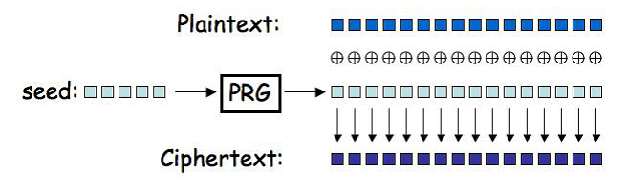
\includegraphics[width=0.7\textwidth]{figures/prg}
\par\end{center}
\begin{mydefinition}[Computational One-Time Pad]
 Let $G:\str n\xrightarrow{}\str{\ell},\ell\gg n$ be a PRG, then
we define a scheme $\left(\enc,\dec\right)$ for $\KK=\str n,\MM=\CC=\str{\ell}$:
\begin{itemize}
\item Choose a secret random short key $k\r\str n$ (\textquotedblplain seed\textquotedblplain )
\item Expand the seed into a long \emph{keying stream }$G\left(k\right)$
\item Encrypt $m$ by $\enc_{k}\left(m\right)=G\left(k\right)\oplus m$
\item Decrypt $c$ by $\dec_{k}\left(c\right)=c\oplus G\left(k\right)$
\end{itemize}
\end{mydefinition}
\begin{thm}
Assume that $\prg:\str n\xrightarrow{}\str{\ell}$ is $\left(t,\varepsilon\right)$-pseudorandom.
Then the \textquotedblplain computational OTP\textquotedblplain{} is
$\left(t-\ell,2\varepsilon\right)$-secure.
\begin{proof}
Let $m_{0},m_{1}\in\MM$, we need to show $\left(\prg\left(\mathcal{U}_{n}\right)\oplus m_{0}\right)\ind{t'}{\varepsilon'}\left(\prg\left(\mathcal{U}_{n}\right)\oplus m_{1}\right)$,
where $t'=t-\ell,\varepsilon'=2\varepsilon$.
\begin{claim}
$\left(\prg\left(\mathcal{U}_{n}\right)\oplus m\right)\ind{t'}{\varepsilon}\left(\mathcal{U}_{\ell}\oplus m\right)\equiv\mathcal{U}_{\ell}$
\end{claim}
From transitivity we conclude $\left(\prg\left(\mathcal{U}_{n}\right)\oplus m_{0}\right)\ind{t'}{\varepsilon'}\left(\prg\left(\mathcal{U}_{n}\right)\oplus m_{1}\right)$.

\textbf{Proof of the claim. }Assume for sake of contradiction there
exists an adversary $\mathcal{A}$ of complexity $t'$ such that $\Delta_{\mathcal{A}}\left(\prg\left(\mathcal{U}_{n}\right)\oplus m_{0},\mathcal{U}_{\ell}\oplus m\right)>\varepsilon$,
we will describe an adversary breaking the PRG.

$\mathcal{A}'\left(z\right)=\mathcal{A}\left(z\oplus m\right)$, and
it's easy to see that $\Delta_{\mathcal{A}'}\left(\prg\left(\mathcal{U}_{n}\right),\mathcal{U}_{\ell}\right)=\Delta_{\mathcal{A}}\left(\prg\left(\mathcal{U}_{n}\right)\oplus m,\mathcal{U}_{\ell}\oplus m\right)>\varepsilon$.

The complexity of $\mathcal{A}'$ is at most $t'+\ell=t$ and thus
we've reached a contradiction.

\end{proof}
\end{thm}
\begin{rem}
PRGs are central primitives in theory of cryptography. If $\P=\NP$
then there are no (polynomial) PRGs, ${\displaystyle L=\left\{ \left.z\left.\colon\right.\exists x.\ \prg\left(x\right)=z\right.\right\} \in\NP}$,
so the existence of PRGs can only be conjectured until $\P\text{ vs }\NP$
is resolved, but we have good reasons to believe they do exist. However
there are good reasons to believe that PRGs do exist. Many candidates
are known whose security can be reduced to seemingly hard problems.
Furthermore, it was shown that PRGs can be constructed based on any
\emph{One-way function}.
\end{rem}

\section{Multiple Messages}
\begin{mydefinition}[Computational Secrecy for Multiple Messages]
 We say $\left(\enc,\dec\right)$ is $\left(t,\varepsilon\right)$-\textbf{computationaly
secrect for multiple messages }if for any $\vec{x}=\left(x_{1},\ldots,x_{n}\right),\vec{y}=\left(y_{1},\ldots,y_{n}\right)\in\MM^{n}$,
s.t. $\left\{ \left(x_{i},y_{i}\right)\right\} _{i=1}^{n}$ are pairs
of equal length messages, if we denote $\vec{c}_{0}=\left(\enc_{k}\left(x_{1}\right),\ldots,\enc_{k}\left(x_{n}\right)\right),c_{1}=\left(\enc_{k}\left(y_{1}\right),\ldots,\enc_{k}\left(y_{n}\right)\right)$
for any $k\in\KK$, then for any adversary $\mathcal{A}$ of complexity
at most $t$:
\[
\Pr_{k\r\KK}\left[\mathcal{A}\left(\vec{c}_{0}\right)=1\right]-\Pr_{k\r\KK}\left[\mathcal{A}\left(\vec{c}_{1}\right)=1\right]<\varepsilon,
\]
i.e. $\vec{c}_{0}\ind t{\varepsilon}\vec{c}_{1}$.
\end{mydefinition}

\subsection{Insecurity}
\begin{thm}
If $\left(\enc,\dec\right)$ is deterministic and dependent on the
key and message $k,m$ only, then it is \emph{insecure for multiple
messages}.
\begin{proof}
Let $a,b\in\MM$ be two different messages of the same length. Then
for
\begin{align*}
\vec{x} & =\left(a,a\right)\\
\vec{y} & =\left(a,b\right)
\end{align*}
we denote where $k\r\KK$, $\vec{c}_{0}=\left(\enc_{k}\left(a\right),\enc_{k}\left(a\right)\right),\vec{c}_{1}=\left(\enc_{k}\left(a\right),\enc_{k}\left(b\right)\right)$.

Let $\mathcal{A}:\mathcal{C}\xrightarrow{}\left\{ 0,1\right\} $ be
defined by $\mathcal{A}\left(z_{1},z_{2}\right)=\mathds{1}\left[z_{1}=z_{2}\right]$,
then
\[
\Pr_{k}\left[\mathcal{A}\left(\vec{c}_{0}\right)=1\right]=1\neq0=\Pr_{k}\left[\mathcal{A}\left(\vec{c}_{1}\right)=1\right]
\]
and thus for any $\varepsilon\in\left[0,1\right]$ one can distinguish
between the distributions, so the scheme is insecure for multiple
messages.
\end{proof}
\end{thm}

\section{Stream Ciphers}
\begin{alg}[From 1-Message Security to Multiple Message Security]
 Let $\left(\enc,\dec\right)$ be secure for single message.
Construct a new scheme with multiple messages security:
\begin{itemize}
\item Initialization: Let $S\r\KK$ be a fresh random key.
\item Encrypt a message $m$ with state $S$:
\begin{itemize}
\item Choose a new random key $S'\r\KK$, send $\enc_{S}\left(m,S'\right)$.
\item Update the state to $S'$.
\end{itemize}
\item To decrypt a ciphertext $c$ with state $S$:
\begin{itemize}
\item Compute $\dec_{S}\left(c\right)=\left(m,S'\right)$, output $m$.
\item Update the new state to $S'$.
\end{itemize}
\end{itemize}
\end{alg}
Alternatively, use a \textbf{stateful PRG}:\\
$\mathrm{PRG}\left(\text{current-state}\right)$ outputs $\left(\text{new-state},\text{pseudorandom-block}\right)$
\begin{alg}[Stream Cipher (Synchronous)]
 Stateful PRGs are the basis for \textbf{stream ciphers:}
\begin{itemize}
\item Let $S_{0}\r\KK$ be the random secrect key, used as the initial state.
\item To encrypt the $i$-th bit of the message $m_{i}$ do:
\begin{itemize}
\item $\left(b_{i},S_{i+1}\right)\xleftarrow{}\prg\left(S_{i}\right)$
\item Output $c_{i}=m_{i}\oplus b_{i}$
\end{itemize}
\end{itemize}
\end{alg}
\begin{prob}
What happens if one bit of the transmission is lost ? 
\end{prob}
\begin{center}
\includegraphics[width=0.45\textwidth]{\string"figures/synchronous stream cipher\string".pdf}
\par\end{center}
\begin{alg}[Asynchronous (Self Synchronizing) Stream Ciphers]
\ 
\begin{itemize}
\item Start with a secret, random key (\textquotedblplain seed\textquotedblplain ),
$k$.
\item Generate online a keying stream.
\item The $i$-th bit is a function of the seed and the recent $t$ bits
of the ciphertext, $\left(c_{i-t},\ldots,c_{i-1}\right)=\text{public state}$.
\item Specifically, encryption is $c_{i}=m_{i}\oplus h\left(k,c_{i-t},\ldots,c_{i-1}\right)$
\item While decryption is $m_{i}=c_{i}\oplus h\left(k,c_{i-t},\ldots,c_{i-1}\right)$
\end{itemize}
\end{alg}

\subsection{Linear Feedback Shift Registers}
\begin{center}
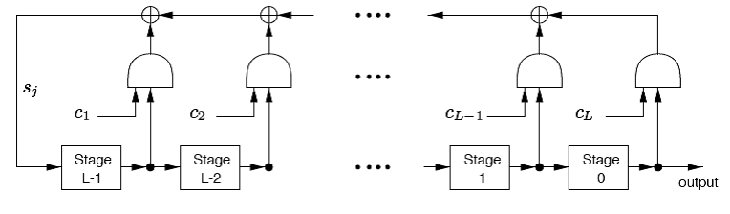
\includegraphics[width=0.7\textwidth]{figures/lfsr}
\par\end{center}
\begin{mydefinition}[Linear Feedback Shift Register]
An \textbf{LFSR} consists of $L$ stages (or delay elements) that
store bits. The device's hardwiring is defined by coefficients $c_{i}\in\{0,1\}$,
with $c_{L}$ always set to$1$.
\begin{itemize}
\item \textbf{Initialization:} The process begins with an initial state
$\left[s_{L-1},\dots,s_{1},s_{0}\right]$.
\item \textbf{Feedback and Output:} The output sequence $s_{0},s_{1},s_{2},\dots$
is determined by a recursion:
\[
s_{j}=\sum_{i=1}^{L}c_{i}s_{j-i}\mod 2
\]
\end{itemize}
\end{mydefinition}
\begin{rem}
With a precise choice of wiring and initialization, the resulting
stream can achieve a very long period.
\end{rem}

\subsection[RC4]{RC4 (Ron's Code 4) }
\begin{alg}[RC4]
 Operates on a state consisting of a permutation $S$ of $\mathbb{Z}_{256}$
and two-8bit index-pointers $i,j$.
\textbf{Initialization:} (Shuffling $S$)
\begin{enumerate}
\item $j=0$
\item $S_{0}=0,S_{1}=1,\ldots,S_{255}=255$
\item Let the key be $k_{0},\ldots,k_{255}$ (repeating bits if key has
fewer bits)
\item For $i=0$ to $255$
\begin{itemize}
\item $j=\left(j+S_{i}+k_{i}\right)\mod{256}$
\item Swap $S_{i}$ and $S_{j}$
\end{itemize}
\end{enumerate}
An output byte $B$ is generated as follows:
\begin{itemize}
\item $i=i+1\mod{256}$
\item $j=j+S_{i}\mod{256}$
\item \emph{Swap }$S_{i}$ and $S_{j}$
\item $r=S_{i}+S_{j}\mod{256}$
\item $B=S_{r}$
\end{itemize}
$B$ is the next keying stream byte, and is XORed with the next plaintext
byte to produce ciphertext byte.
\end{alg}

\section[CPA Security]{Indistinguishability under Chosen Plaintext Attack}
\begin{thm}[Ciphertext Indistinguishability: Alternative Definition]
 Consider the following game:

\begin{center}
\begin{tikzpicture}]

    % --- Challenger ---
    \node[chalbox] (C) at (-2.5,0) {
        \textbf{Challenger}\\
        $k \r \KK$\\[0.25em]
        $b \r \binary$\\
    };

    % --- Adversary ---
    \node[advbox] (A) at (2.5,0) {
        \textbf{Adversary $\mathcal{A}$}\\[3em]
        \textcolor{red}{Output $b'$}
    };

    % --- Communication ---
    \draw[arrow] ([yshift=1em]A.west) -- node[above] {$(m_0, m_1)$} ([yshift=1em]C.east);
    \draw[arrow] ([yshift=-1em]C.east) -- node[below] {$\enc_k(m_b)$} ([yshift=-1em]A.west);

\end{tikzpicture}
\end{center}

Then, $\left(\enc,\dec\right)$ has $\left(t,\varepsilon\right)$-computational
secrecy if and only for every $t$-time adversary $\Pr\left[b'=b\right]\leq\frac{1}{2}+\frac{1}{2}\varepsilon$.
\end{thm}
Proof: HW1, Q2.
\begin{mydefinition}[Indistinguishability under Chosen Plaintext Attack]
 Consider the following game:

\begin{center}
\begin{tikzpicture}]

    % --- Challenger ---
    \node[chalbox] (C) at (-2.5,0) {
        \textbf{Challenger}\\
        $k \r \KK$\\[3.25em]
        $b \r \binary$\\
    };

    % --- Adversary ---
    \node[advbox] (A) at (2.5,0) {
        \textbf{Adversary $\mathcal{A}$}\\[6em]
        \textcolor{red}{Output $b'$}
    };

	\node[color=blue] at (0,0) {$\vdots$};
    % --- Communication ---
    \draw[arrow, color=blue] ([yshift=2.5em]A.west) -- node[above] {$x_1$} ([yshift=2.5em]C.east);
    \draw[arrow, color=blue] ([yshift=2em]C.east) -- node[below] {$\enc_k(x_1)$} ([yshift=2em]A.west);
	\draw[arrow, color=red] ([yshift=-2.5em]A.west) -- node[above] {$\left(m_0,m_1\right)$} ([yshift=-2.5em]C.east);
    \draw[arrow, color=red] ([yshift=-3em]C.east) -- node[below] {$\enc_k(m_b)$} ([yshift=-3em]A.west);
	
\end{tikzpicture}
\end{center}

The game has two phases:
\begin{enumerate}
\item $\mathcal{A}$ is allowed to \textcolor{blue}{adaptively choose many
encryptions}
\item $\mathcal{A}$ chooses a test $m_{0},m_{1}\in\MM$ and tries to \textcolor{red}{distinguish
}$\enc_{k}\left(m_{0}\right)$ from $\enc_{k}\left(m_{1}\right)$
\end{enumerate}
We then say, $\left(\enc,\dec\right)$ is $\left(t,\varepsilon\right)$-\textbf{CPA
secure }if for every $t$-time adversary $\Pr\left[b'=b\right]\leq\frac{1}{2}+\varepsilon$.
\end{mydefinition}

\subsection{Random Encryption}
\begin{mydefinition}[Random Function]
 We say $R:\Omega\times\mathcal{X}\xrightarrow{}\mathcal{Y}$ is
a \textbf{random function}, if for any $x\in\mathcal{X}$, $R\left(x\right)\coloneqq R\left(\cdot,x\right):\Omega\xrightarrow{}\mathcal{Y}$
is a uniform RV.
\end{mydefinition}
%
\begin{mydefinition}[Random Permutation]
 We say $R:\Omega\times\mathcal{X}\xrightarrow{}\mathcal{X}$ is
a \textbf{random permutation }if it is uniformly distributed over
all permutations on $\mathcal{X}$. (i.e. a random function conditioned
on it being a permutation.)
\end{mydefinition}
\begin{alg}[Encryption From Permutation]
 Let $F:\str n\xrightarrow{}\str n$ be a permutation (maybe random)
on $\str n$.
\begin{itemize}
\item Encrypt $m$: choose $r\r\str n$ and output $\enc\left(m\right)=\left(r,F\left(r\oplus m\right)\right)$
\item Decrypt $\left(r,c\right)$: compute $\dec\left(c\right)=r\oplus F^{-1}\left(c\right)$
\end{itemize}
\end{alg}
\begin{thm}
If $F$ is random, then the scheme above is $\left(t,\varepsilon\right)$-CPA
secure where $\varepsilon=O\left(t/2^{n}\right)$.
\begin{proof}
\ 
\begin{itemize}
\item For $i\in\left[t\right]$: Adversary $\mathcal{A}$ sends $x_{i}$
and gets $\left(r_{i},c_{i}=F\left(x_{i}\oplus r_{i}\right)\right)$.
\item The challenge $m_{b}$ is encrypted by $\left(r_{*},c_{*}=F\left(m_{b}\oplus r_{*}\right)\right)$.
\item Call $r_{*}$ \emph{good }if $m_{0}\oplus r_{*}$ and $m_{1}\oplus r_{*}$
are not in $\left\{ x_{i}\oplus r_{i}\right\} _{i\in\left[t\right]}$.
\item $\Pr\left[r_{*}\text{ is good}\right]\geq1-2t/2^{n}$.
\item Conditioned on being good, $\mathcal{A}$ can't win with prob. larger
than $1/2$.
\item Since $r_{*}$ is uniform over good \& $c_{*}$ is uniform over $\str n\setminus\left\{ c_{i}\right\} _{i\in\left[t\right]}$,
regardless of the value of $b$.
\end{itemize}
\end{proof}
\end{thm}
\begin{prob}
Alice and Bob can't share a random function (too expensive).
\end{prob}

\section[PRFs and PRPs ]{Pseudorandom Functions and Permutations }
\begin{mydefinition}[Collection of Functions]
 $F:\KK\times\mathcal{X}\xrightarrow{}\mathcal{X}$,we denote for
each $k\in\KK$, $F\left(k,\cdot\right)=F_{k}:\mathcal{X}\xrightarrow{}\mathcal{X}$.
\end{mydefinition}
%
\begin{mydefinition}[Collection of Permutations]
 $F:\KK\times\mathcal{X}\xrightarrow{}\mathcal{X}$ where for all
$k\in\KK$, $F_{k}$ is a \emph{permutation}.
\end{mydefinition}
%
\begin{mydefinition}[Pseudorandom Functions (GoldreichGoldwasserMicali84)]
 We say $F:\KK\times\mathcal{X}\xrightarrow{}\mathcal{X}$ is a $\left(t,\varepsilon\right)$-\textbf{pseudorandom
function }if for any $x\in\mathcal{X}$, if $k\r\KK$ and $R:\mathcal{X}\xrightarrow{}\mathcal{X}$
is random, then $F_{k}\left(x\right)\ind t{\varepsilon}R\left(x\right)$.
\end{mydefinition}
\begin{thm}[PRFs: Equivalent Definition]
 Let $F:\KK\times\mathcal{X}\xrightarrow{}\mathcal{X}$, and consider
the following game:

\begin{center}
\begin{tikzpicture}]

    % --- Challenger ---
    \node[chalbox] (C) at (-2.5,0) {
        \textbf{Challenger}\\
        $k \r \KK$\\
        $b \r \binary$\\
		If $b=0$:\\
		set $R\coloneqq F_k$\\
		Else: sample\\ random $R$
    };

    % --- Adversary ---
    \node[advbox] (A) at (2.5,0) {
        \textbf{Adversary $\mathcal{A}$}\\[7.25em]
        \textcolor{red}{Output $b'$}
    };

	\node at (0,-3em) {$\vdots$};
    % --- Communication ---
    \draw[arrow] ([yshift=3.5em]A.west) -- node[above] {$x_1$} ([yshift=3.5em]C.east);
    \draw[arrow] ([yshift=3em]C.east) -- node[below] {$R(x_1)$} ([yshift=3em]A.west);
	\draw[arrow] ([yshift=0.25em]A.west) -- node[above] {$x_2$} ([yshift=0.25em]C.east);
    \draw[arrow] ([yshift=-0.25em]C.east) -- node[below] {$R(x_2)$} ([yshift=-0.25em]A.west);
	
\end{tikzpicture}
\end{center}

Then $F$ is $\left(t,\varepsilon\right)$-pseudorandom if and only
if for any $t$-timed adversary $\Pr\left[b'=b\right]\leq\frac{1}{2}+\varepsilon$.
\end{thm}
\begin{mydefinition}[PRP]
 A collection of permutations $F$ is a $\left(t,\varepsilon\right)$-\textbf{pseudorandom
permutation }if the above holds where we sample a random permutation
$R$.
\end{mydefinition}
%
\begin{mydefinition}[Strong PRP]
A collection of permutations $F$ is a $\left(t,\varepsilon\right)$-\textbf{strong
pseudorandom permutation }if the above holds where we sample a random
permutation $R$, and the adversary can also query $R^{-1}$.
\end{mydefinition}

\subsection[CPA Security from PRP]{CPA Security from Pseudorandom Permutation}
\begin{alg}[Encryption from PRP]
 Let $F:\KK\times\str n\xrightarrow{}\str n$ be a PRP on $\str n$.
\begin{itemize}
\item Encrypt $m$: choose $r\r\str n$ and output $\enc_{k}\left(m\right)=\left(r,F_{k}\left(r\oplus m\right)\right)$
\item Decrypt $\left(r,c\right)$: compute $\dec_{k}\left(c\right)=r\oplus F_{k}^{-1}\left(c\right)$
\end{itemize}
\end{alg}
\begin{thm}
If $F$ is $\left(t,\varepsilon\right)$-pseudorandom the scheme above
is $\left(\Omega\left(t/n\right),2\varepsilon+t/2^{n}\right)$-CPA
secure.
\begin{proof}
The proof proceeds by \emph{reduction}. We assume towards contradiction
that there exists an adversary $\mathcal{A}_{\enc}$ that wins the
CPA game with prob. $0.5+\delta$. We construct an adversary $\mathcal{A}_{\prf}$
that wins the PRF game.

\begin{center}
\begin{tikzpicture}[node distance=2.5cm]

    % --- 1. PRF Challenger (The Oracle) ---
    \node[chalbox, minimum height=4.5cm] (C) at (-6,0) {
        \textbf{PRF Challenger}\\
        $k \leftarrow \mathcal{K}, b \leftarrow \{0,1\}$\\
        $R\gets\begin{cases}F_{k}, & b=0\\\text{random}, & b=1\end{cases}$
    };

    % --- 2. PRF Adversary (The Simulator) ---
    \node[box, fill=gray!5, draw=black, minimum height=5.5cm, minimum width=3.5cm] (PRF) at (0,0) {
		$r_i \r \str{n}$\\
        \textbf{PRF Adversary}\\
        $\mathcal{A}_{\prf}$
    };

    % --- 3. Enc Adversary (The Target) ---
    \node[advbox, minimum height=4.5cm] (Enc) at (5.5,0) {
        \textbf{Enc Adversary}\\
        $\mathcal{A}_{\enc}$
    };

    % --- Interaction 1: Queries (Top) ---
    \draw[arrow] ([yshift=1.375cm]Enc.west) -- node[above] {$x_i$} ([yshift=1.375cm]PRF.east);
    \draw[arrow] ([yshift=1.375cm]PRF.west) -- node[above] {$a_i=r_i \oplus x_i$} ([yshift=1.375cm]C.east);
    \draw[arrow] ([yshift=1.125cm]C.east) -- node[below] {$y_i=R(a_i)$} ([yshift=1.125cm]PRF.west);
    \draw[arrow] ([yshift=1.125cm]PRF.east) -- node[below] {$(r_i, y_i)$} ([yshift=1.125cm]Enc.west);

    \node at (3, 0) {$\vdots$};
    \node at (-3, 0) {$\vdots$};

    % --- Interaction 2: Challenge (Bottom) ---
    \draw[arrow] ([yshift=-1.125cm]Enc.west) -- node[above] {$m_0, m_1$} ([yshift=-1.125cm]PRF.east);
    \draw[arrow] ([yshift=-1.125cm]PRF.west) -- node[above] {$r^* \oplus m_{b^*}$} ([yshift=-1.125cm]C.east);
    \draw[arrow] ([yshift=-1.375cm]C.east) -- node[below] {$y^*$} ([yshift=-1.375cm]PRF.west);
    \draw[arrow] ([yshift=-1.375cm]PRF.east) -- node[below] {$(r^*, y^*)$} ([yshift=-1.375cm]Enc.west);

    % --- Final Outputs ---
    \draw[arrow] (Enc.south) -- ++(0,-0.5) node[below] {Output $\tilde{b}$};
    \draw[arrow] (PRF.south) -- ++(0,-0.5) node[below, color=red] {Output $b' = (b^* \neq \tilde{b})$};

\end{tikzpicture}
\end{center}

If $b=0$, $\Pr\left[b'=0\right]=\Pr\left[\mathcal{A}_{\enc}\text{ wins}\right]=0.5+\delta$.

If $b=1$, $\Pr\left[b'=0\right]=\Pr\left[\mathcal{A}_{\enc}\text{ wins against random function}\right]=0.5+t2^{-n}$.

All in all, $\Pr\left[b'=b\right]\geq0.5+0.5\left(\delta-t2^{-n}\right)$,
and thus for $\delta=2\varepsilon+t/2^{n}$ we get a contradiction,
since the complexity of $\mathcal{A}_{\prf}$ is that of $\mathcal{A}_{\enc}$
times $n$ because XORing a string takes $O\left(n\right)$.
\end{proof}
\end{thm}


\chapter{Block Ciphers}


\section[Block Ciphers]{PRPs in Practice: Block Ciphers}
\begin{mydefinition}[Block Cipher]
 A \textbf{block cipher }is a implementation of a keyed pseudorandom
permutation, with $\KK=\str n$.
\end{mydefinition}
\begin{rem}
To encrypt messages longer than $n$, you divide the message to $n$-bit
blocks (maybe expand the last), and then encrypt as
\[
\enc_{k}\left(m\right)=\left(\left(r_{1},F_{k}\left(r_{1}\oplus m_{1}\right)\right),\ldots,\left(r_{t},F_{k}\left(r_{t}\oplus m_{t}\right)\right)\right)
\]
\end{rem}
%
\begin{rem}
A block cipher is \textbf{not }an encryption scheme, modes of operations
are \textquotedblplain wrappers\textquotedblplain{} that turns a block
cipher into a full-fledged encryption scheme.
\end{rem}

\section{Modes of Operation}

\subsection[CBC]{Cipher Block Chaining}
\begin{alg}[CBC]
In CBC mode (Cipher Block Chaining), previous ciphertext is XORed
with current plaintext before encrypting current block.
\begin{center}
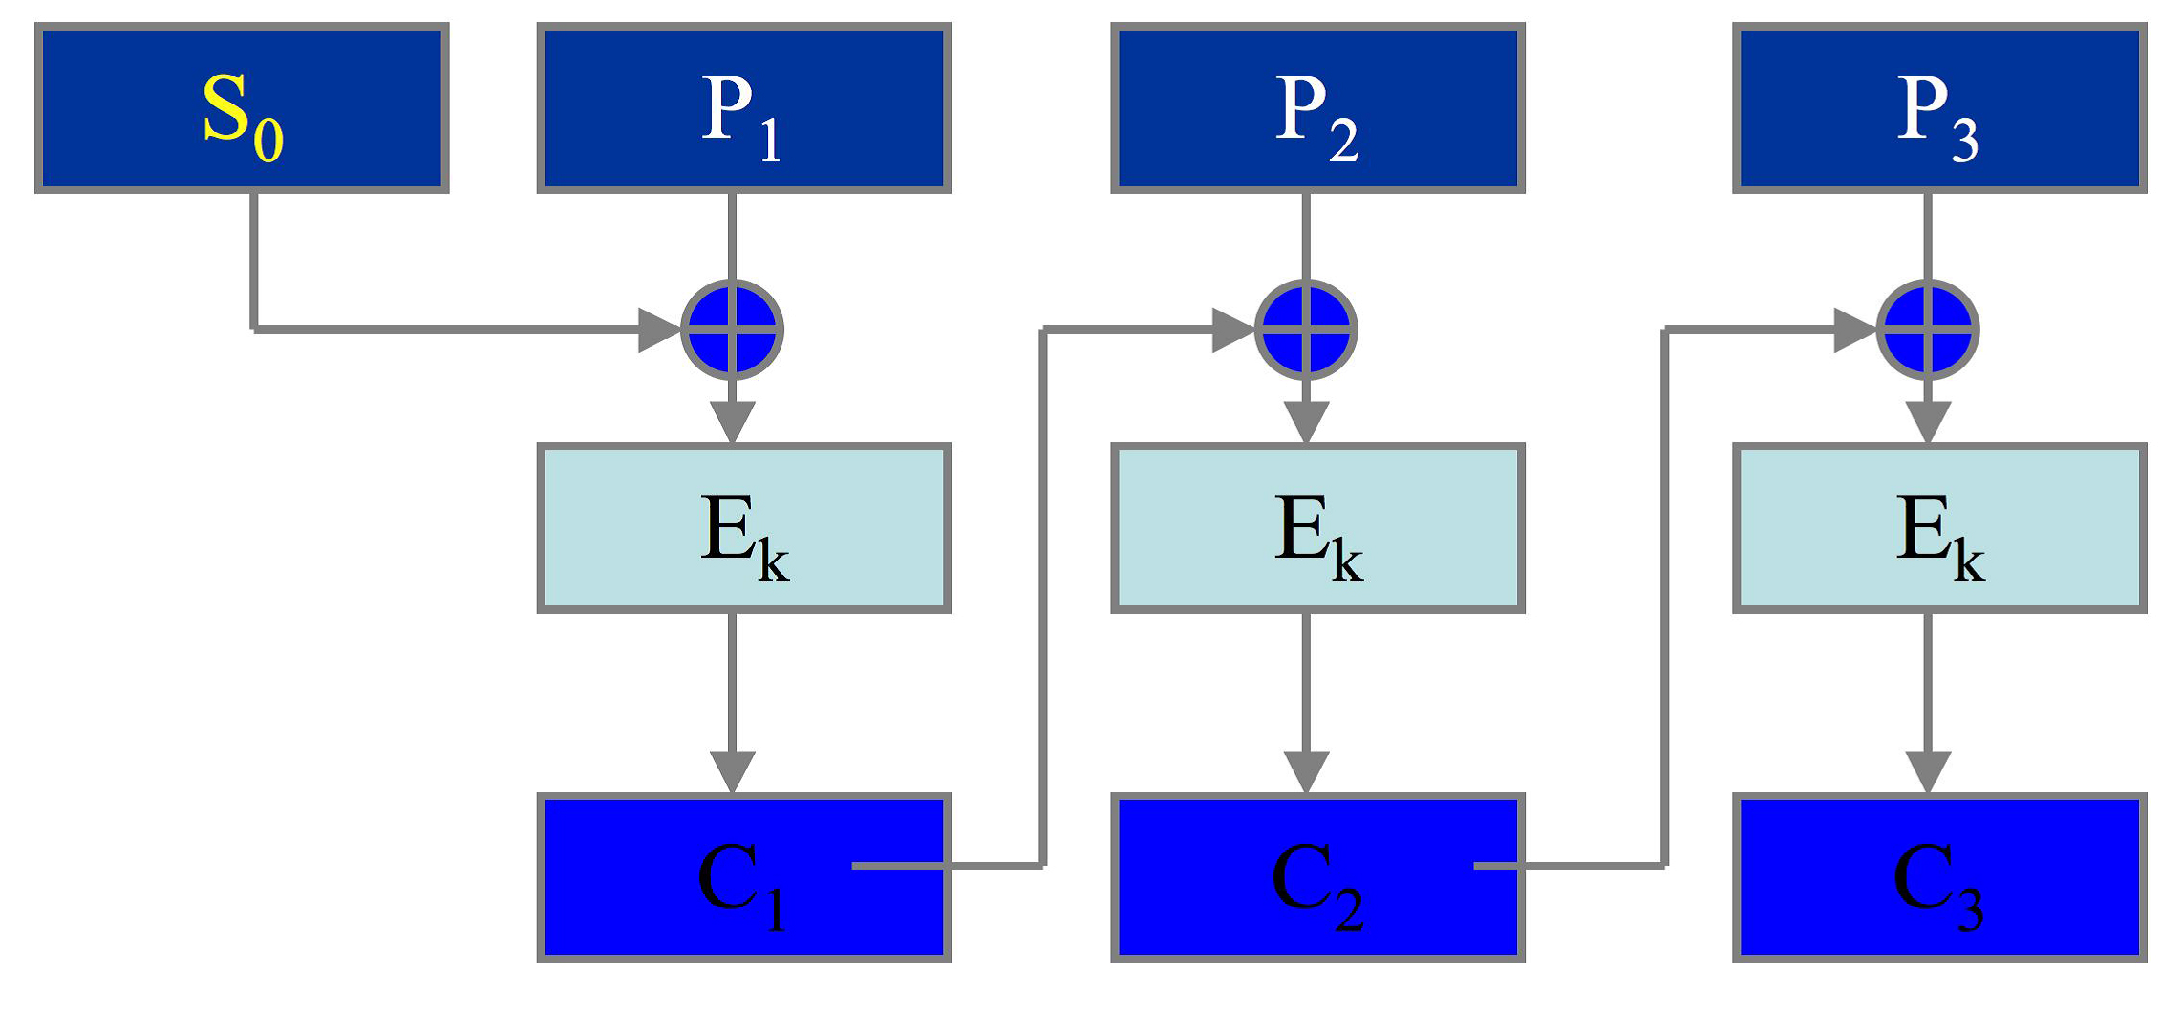
\includegraphics[width=0.6\textwidth]{figures/cbc}
\par\end{center}
\begin{itemize}
\item $S_{0}$ is an \emph{initialization vector }(IV) used as a \textquotedblplain seed\textquotedblplain{}
for the process which is openly transmitted
\item To ensure security, each message should have a new random vector as
a seed
\end{itemize}
\end{alg}
\begin{claim}
If $E$ is a PRP then CBC is CPA-secure.
\end{claim}

\subsection[OFB]{Output Feedback}
\begin{alg}[OFB]
\ 
\begin{itemize}
\item An initialization vector $S_{0}$ is use as a \textquotedblplain seed\textquotedblplain{}
for a sequence of pseudorandom blocks $S_{1},S_{2},\ldots$
\item Each $S_{i}$ is XORed with the $i$-th plaintext block $P_{i}$ to
produce the $i$-th ciphertext block $C_{i}$.
\item It is important to use a new random seed for each message.
\end{itemize}
\begin{center}
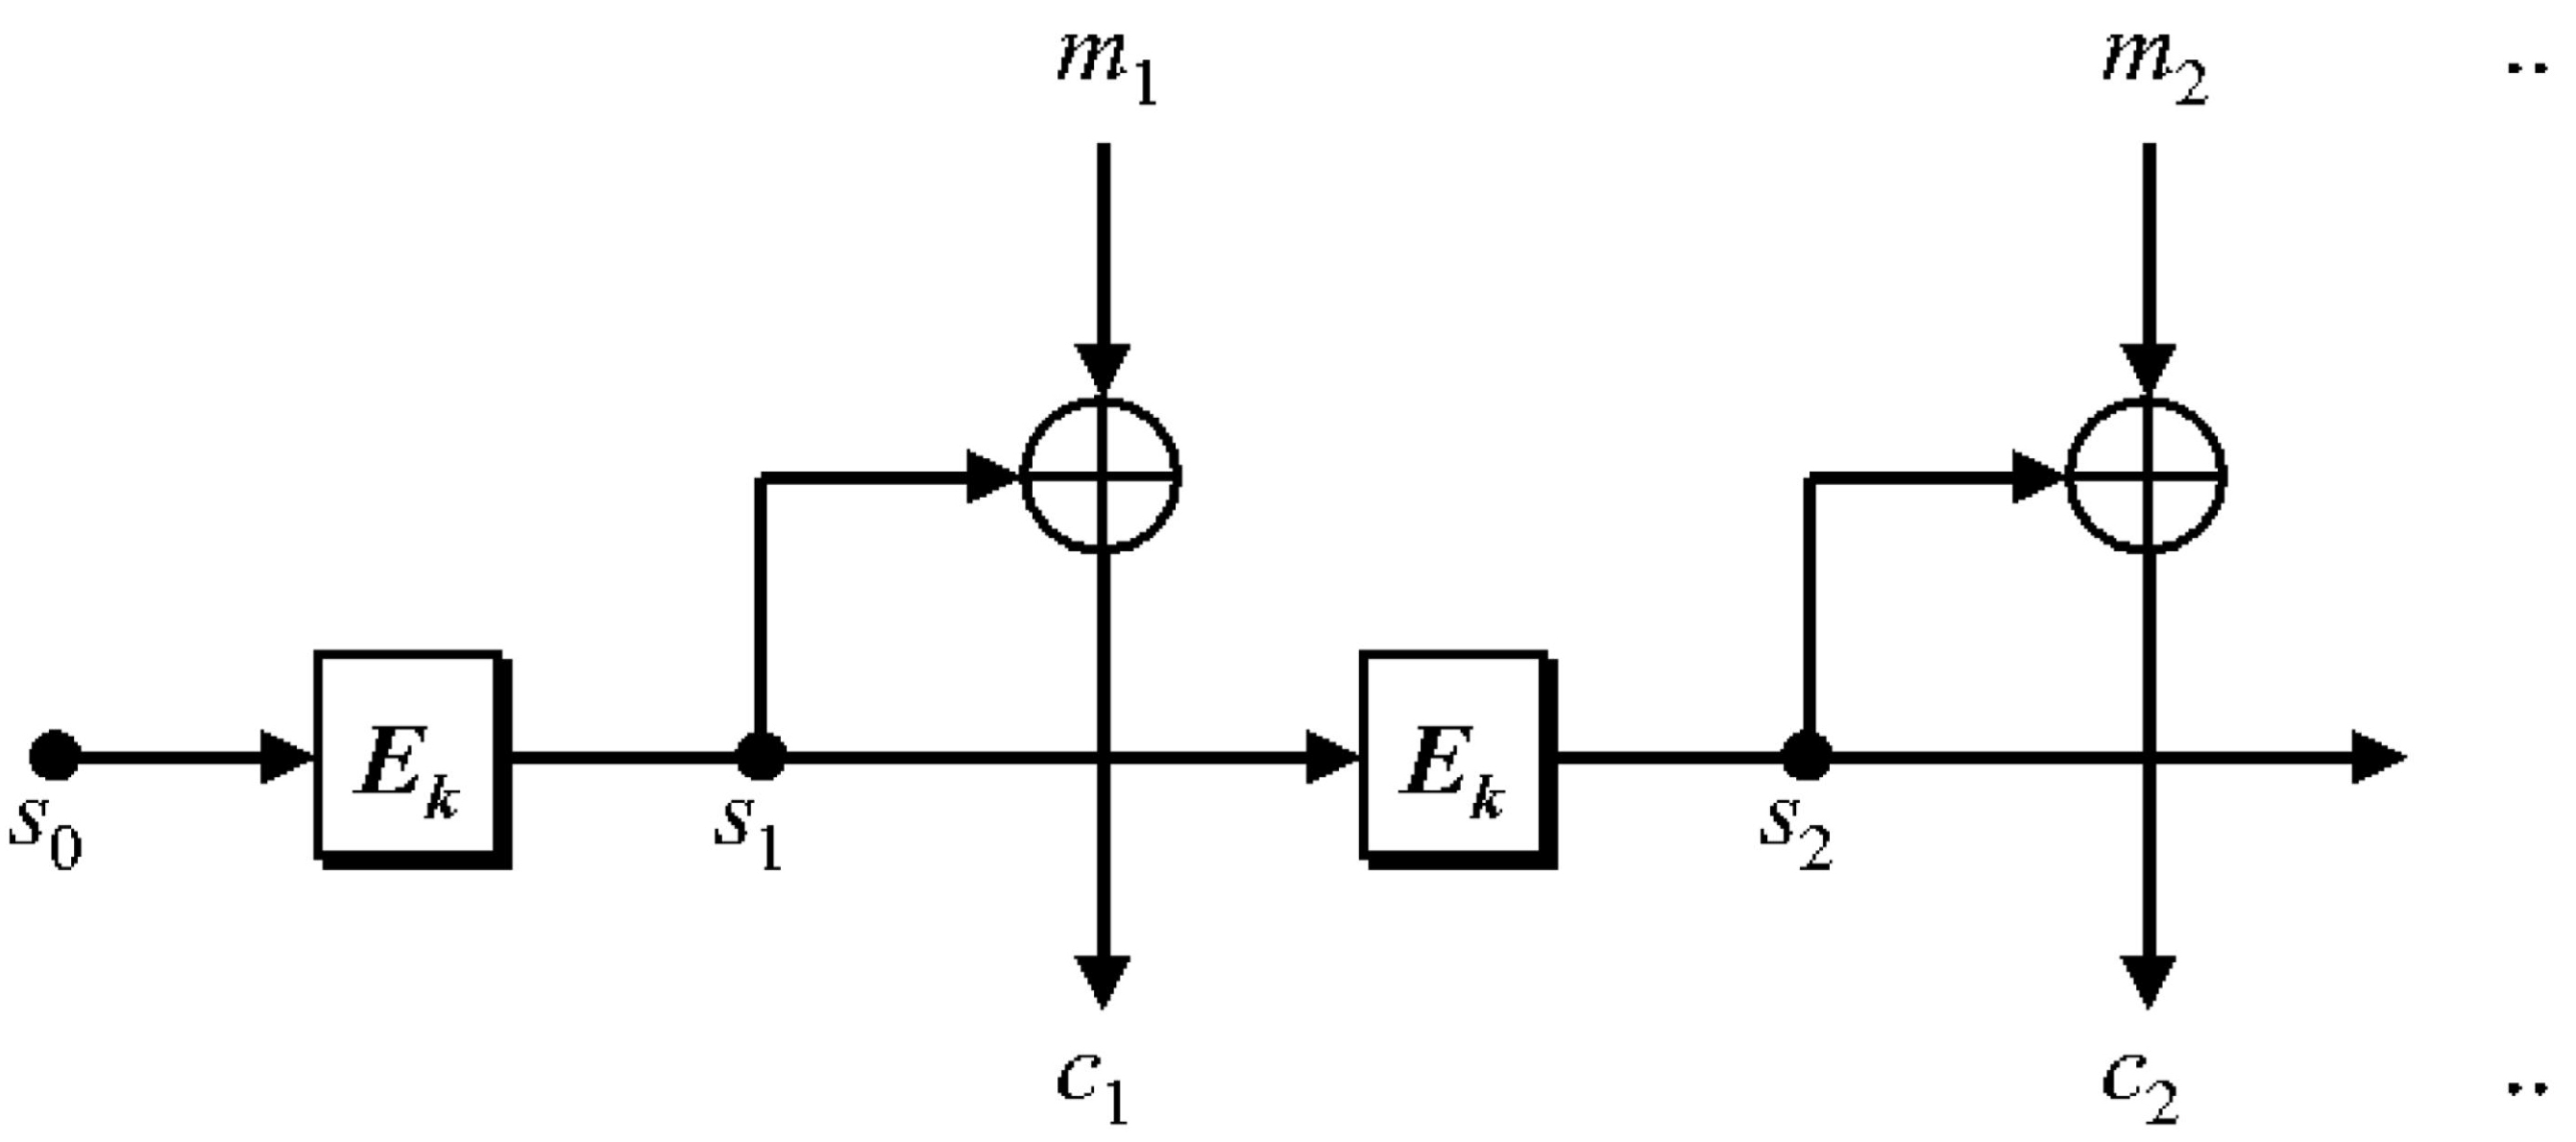
\includegraphics[width=0.7\textwidth]{figures/OFB}
\par\end{center}

\end{alg}
\begin{claim}
If $E$ is a PRF then OFB is CPA-secure.
\end{claim}

\subsection[ECB]{Electronic Code Book}
\begin{alg}[ECB]
Simplest mode is to encrypt each plaintext block separately. This
is known as ECB mode encryption (Electronic Code Book).
\begin{center}
\includegraphics[width=0.5\textwidth]{figures/ecb}
\par\end{center}

\end{alg}
\begin{claim}
ECB is not CPA-secure (even if $E$ is pseudorandom).
\end{claim}

\section[Feistel Networks]{Feistel Networks: Important Building Block in DES}

\begin{center}
\begin{tikzpicture}[node distance=1.5cm, >=Stealth]
    % Coordinates for the round
    \node (Li_prev) at (-2, 1.5) {$L_{i-1}$};
    \node (Ri_prev) at (2, 1.5) {$R_{i-1}$};
    
    % XOR and Function nodes
    \node[draw, minimum width=1.2cm, fill=blue!5] (f) at (0, 0.5) {$f$};
    \node[circle, draw, inner sep=0pt, minimum size=0.4cm] (xor) at (-2, 0.5) {};
    \draw (-2, 0.5) -- ++(0, 0.2) -- ++(0, -0.4); 
    \draw (-2, 0.5) -- ++(0.2, 0) -- ++(-0.4, 0); 
    
    \node (ki) at (0, 1.5) {$k_i$};
    
    % Outputs
    \node (Li) at (-2, -1) {$L_i$};
    \node (Ri) at (2, -1) {$R_i$};

    % Connections
    \draw[->] (Ri_prev.south) -- (2, 0.5) -- (f.east);
    \draw[->] (f.west) -- (xor.east);
    \draw[->] (Li_prev) -- (xor.north);
    \draw[->] (ki) -- (f.north);
    
    % The Feistel Swap logic
    \draw[->] (xor.south) -- (-2, 0) -- (2, -0.2) -- (Ri.north);
    \draw[->] (2, 0.5) -- (2, 0) -- (-2, -0.2) -- (Li.north);
\end{tikzpicture}
\end{center}
\begin{alg}[Feistel Round Function]
 To compute the $i$-th Feistel round on an input $\left(L_{0},R_{0}\right)\in\str{2n}$
for a function collection $f:\KK\times\str n\xrightarrow{}\str n$:
\begin{enumerate}
\item \textbf{Recursion: }Compute $\left(L_{i-1},R_{i-1}\right)\in\str{2n}$
\item \textbf{Function Application: }Compute $f\left(k_{i},R_{i-1}\right)$
using the $i$-th part of the key $k_{i}$
\item \textbf{XOR \& Swap: }$L_{i}\xleftarrow{}R_{i-1},R_{i}\xleftarrow{}L_{i-1}\oplus f\left(k_{i},R_{i-1}\right)$
\item Return $F_{i}\left(L_{0},R_{0}\right)=\left(L_{i},R_{i}\right)$
\end{enumerate}
\end{alg}
\begin{claim}
For any $f:\KK\times\str n\xrightarrow{}\str n$, and any $i\in\mathbb{N}$,
$F_{i}:\str{2n}\xrightarrow{}\str{2n}$ is a permutation on $\str{2n}$.
\end{claim}
\begin{thm}[Luby-Rackoff '88]
 If $f$ is a PRF then a \emph{four-round} Feistel network using
independent keys for each round yields a PRP.
\end{thm}
%
\begin{thm}[Failure of 2-Round Feistel]
 A two-round Feistel network $G:\str{2n}\rightarrow\str{2n}$ constructed
from secure PRFs $F_{1},F_{2}$ is not a PRF.
\end{thm}
Proof: HW2, Q4.

\section[AES]{AES Encryption/Decryption: Carried out in Ten Rounds}

Advanced Encryption Standard (AES) operates by the following:
\begin{flushleft}
\begin{tabular}[b]{V{\linewidth}cc}
\begin{itemize}
\item Input \& output block length: 128 bits.
\item State: 128 bits, arranged in a 4-by-4 matrix of bytes.
\item Each byte is viewed as an element in $GF\left(2^{8}\right)$.
\end{itemize}
 & \multirow{1}{*}{%
\begin{tabular}{|c|c|c|c|}
\hline 
$S_{0,0}$ & $S_{0,1}$ & $S_{0,2}$ & $S_{0,3}$\tabularnewline
\hline 
$S_{1,0}$ & $S_{1,1}$ & $S_{1,2}$ & $S_{1,3}$\tabularnewline
\hline 
$S_{2,0}$ & $S_{2,1}$ & $S_{2,2}$ & $S_{2,3}$\tabularnewline
\hline 
$S_{3,0}$ & $S_{3,1}$ & $S_{3,2}$ & $S_{3,3}$\tabularnewline
\hline 
\end{tabular}} & \tabularnewline
\end{tabular}
\par\end{flushleft}

128 bits AES uses 10 rounds. These are not Feistel rounds.
\begin{itemize}
\item The secret key is expanded from 128 bits to 10 round keys, 128 bits
each.
\item Each round changes the state, then XORS the round key.
\end{itemize}
Each rounds complicates things a little. Overall it seems infeasible
to invert without the secret key (but easy given the key).

\subsection{AES Specifications: One Round}

Transform the state by applying:
\begin{enumerate}
\item Substitution: operates on every byte separately: $S_{i,j}\xleftarrow{}S_{i,j}^{-1}$\\
(multiplicative inverse in$GF\left(2^{8}\right)$, which is highly
non-linear).\\
If $S_{i,j}=0$, don't change it.\\
Clearly, the substitution is invertible.
\item Cyclic Shift inside Rows: Clearly, the shift is invertible,
\begin{center}
\begin{tabular}{|c|c|c|c||c|}
\hline 
$S_{0,0}$ & $S_{0,1}$ & $S_{0,2}$ & $S_{0,3}$ & (no shift)\tabularnewline
\hline 
$S_{1,3}$ & $S_{1,0}$ & $S_{1,1}$ & $S_{1,2}$ & (shift one position)\tabularnewline
\hline 
$S_{2,2}$ & $S_{2,3}$ & $S_{2,0}$ & $S_{2,1}$ & (shift two positions)\tabularnewline
\hline 
$S_{3,1}$ & $S_{3,2}$ & $S_{3,3}$ & $S_{3,0}$ & (shift three positions)\tabularnewline
\hline 
\end{tabular}
\par\end{center}
\item MixCol: maps the state to a new one.\\
It multiplies each column of state by the polynomial $c\left(x\right)\mod{\left(x^{4}+1\right)}$,
where
\[
c\left(x\right)=\texttt{0x03}x^{3}+\texttt{0x01}x^{2}+\texttt{0x01}x+\texttt{0x02}.
\]
Specifically, for the first column,
\[
S_{0,0}'x^{3}+S_{1,0}'x^{2}+S_{2,0}'x+S_{3,0}'=\left(\texttt{0x03}x^{3}+\texttt{0x01}x^{2}+\texttt{0x01}x+\texttt{0x02}\right)\cdot\left(S_{0,0}x^{3}+S_{1,0}x^{2}+S_{2,0}x+S_{3,0}\right)\mod{\left(x^{4}+1\right).}
\]
The inverse operation is InvMixCol: It multiplies each column of state
by the polynomial $d\left(x\right)\mod{\left(x^{4}+1\right)}$, where
\[
d\left(x\right)=\texttt{0x0b}x^{3}+\texttt{0x0d}x^{2}+\texttt{0x09}x+\texttt{0x0e}.
\]

\begin{rem}
All these coefficients from $c(x)$ and $d(x)$ ($\texttt{0x03,0x01,0x02,0x0b,0x0d,0x09,0x0e}$)
are hexadecimal constants from $GF\left(2^{8}\right)$ (which are
low degree polynomials, e.g. $\texttt{0x0e}$ in hex is 14 in decimal,
1110 in binary, and $x^{3}+x^{2}+x$ as a polynomial).
\end{rem}
%
\begin{rem}
These $c(x)$ and $d(x)$ correspond to the first (left most) column.
The other columns have different but similar coefficients/polynomials.
\end{rem}
\begin{center}
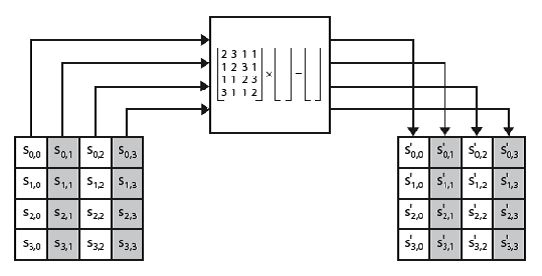
\includegraphics[width=0.7\textwidth]{figures/mixcol}
\par\end{center}
\item XOR round key: not discussed.
\end{enumerate}
\begin{center}
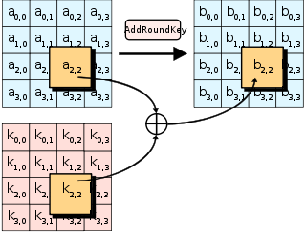
\includegraphics[width=0.5\textwidth]{figures/aes}
\par\end{center}

\begin{center}
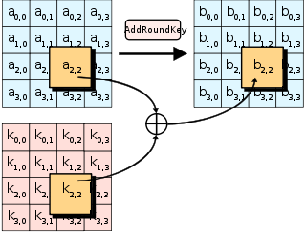
\includegraphics[width=0.7\textwidth]{figures/aes}
\par\end{center}

\section{Strengthening a Given Block Cipher}

\subsection{Double Ciphers}

\textbf{Idea:} Double-encryption. Instead of using a single key, $k$,
use two keys, $k_{1},k_{2}$.
\begin{center}

\includegraphics[width=0.5\textwidth]{figures/itciph}
\par\end{center}

\textbf{Hope:} Complexity of exhaustive attack grow from$O\left(2^{n}\right)$
to $O\left(2^{2^{n}}\right)$, where $n$ is the original key-length.
\begin{rem}
If an encryption is closed under composition then iterating it for
any number of times is pointless.

That is, if for all $k_{1},k_{2}$ there is $k_{3}$ such that $\enc_{k_{2}}\left(\enc_{k_{1}}\left(x\right)\right)=\enc_{k_{3}}\left(x\right)$,
then we could just exhaustively search for such $k_{3}$.

then we could just exhaustively search for such k3.
\end{rem}

\subsubsection{Ideal Ciphers}
\begin{center}

\includegraphics[width=0.5\textwidth]{figures/itciph}
\par\end{center}

The \emph{ideal cipher model}:
\begin{itemize}
\item For every $k\in\str n$ sample a random permutation $\enc_{k}$ on
$\str n$ and let $\dec_{k}$ denote its inverse.
\item Evaluating $\enc_{k},\dec_{k}$ for any given key $k$ is a unit-cost
operation.
\end{itemize}
\emph{The attack model: }A pair $\left(k_{1},k_{2}\right)$ of random
keys is sampled uniformly. Our goal is to recover the keys given oracle
access to the encryption scheme.

\subsubsection{Meet in the Middle Attack}
\begin{center}

\includegraphics[width=0.5\textwidth]{figures/meetinthemiddle}
\par\end{center}

\textbf{Goal: }Recover the two keys $k_{1},k_{2}$.
\begin{enumerate}
\item Ask for a pair of plaintext/ciphertext $\left(x,y\right)$ for the
new scheme, i.e., $\left(\enc_{k_{2}}\circ\enc_{k_{1}}\right)\left(x\right)=y$.
\item Find all candidates $\left(k,k'\right)$ for which $\enc_{k}\left(x\right)=\dec_{k'}\left(y\right)$.
\begin{itemize}
\item How many such pairs exist? $O\left(2^{n}\right)$ in expectation.
\end{itemize}
\item Use another plaintext/ciphertext pair $\left(x',y'\right)$ to filter
out inconsistent candidates. Whp, only the right key survives. (If
not, use another pair).
\end{enumerate}
\begin{alg}
For each key $k$ store $\enc_{k}\left(x\right)$ in list $L_{1}$
and store $D_{k}\left(y\right)$ in $L_{2}$, sort lists in time $O\left(n2^{n}\right)$
and find intersection in time $O\left(2^{n}\right)$.
\end{alg}

\paragraph{Meet in the Middle Attack: Performance}

\textbf{Time: }$O\left(n2^{n}\right)$, \textbf{Space: }$O\left(2^{n}\right)$

Compare this to exhaustive search over the space of a\emph{ single}
key:

\textbf{Time: }$O\left(n2^{n}\right)$, \textbf{Space: }$O\left(1\right)$
\begin{conc}
Double cipher (two iterations) does not add much to security (though
it adds some, esp. if fast memory is expensive).
\end{conc}

\subsection{Triple Cipher}
\begin{center}
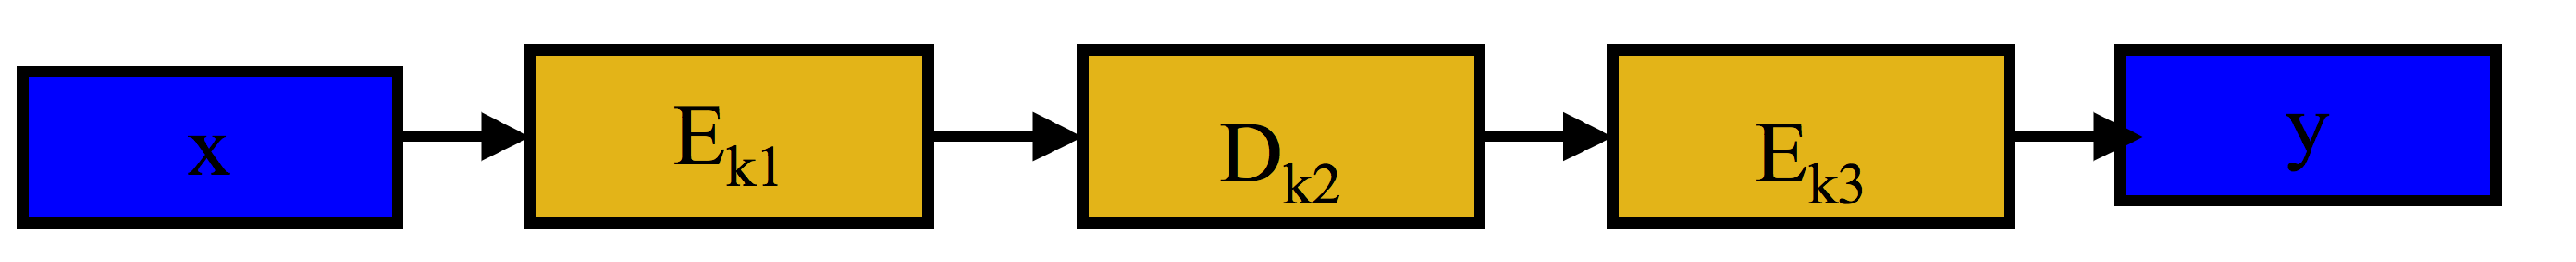
\includegraphics[width=0.5\textwidth]{figures/tcip1}
\par\end{center}

\begin{center}
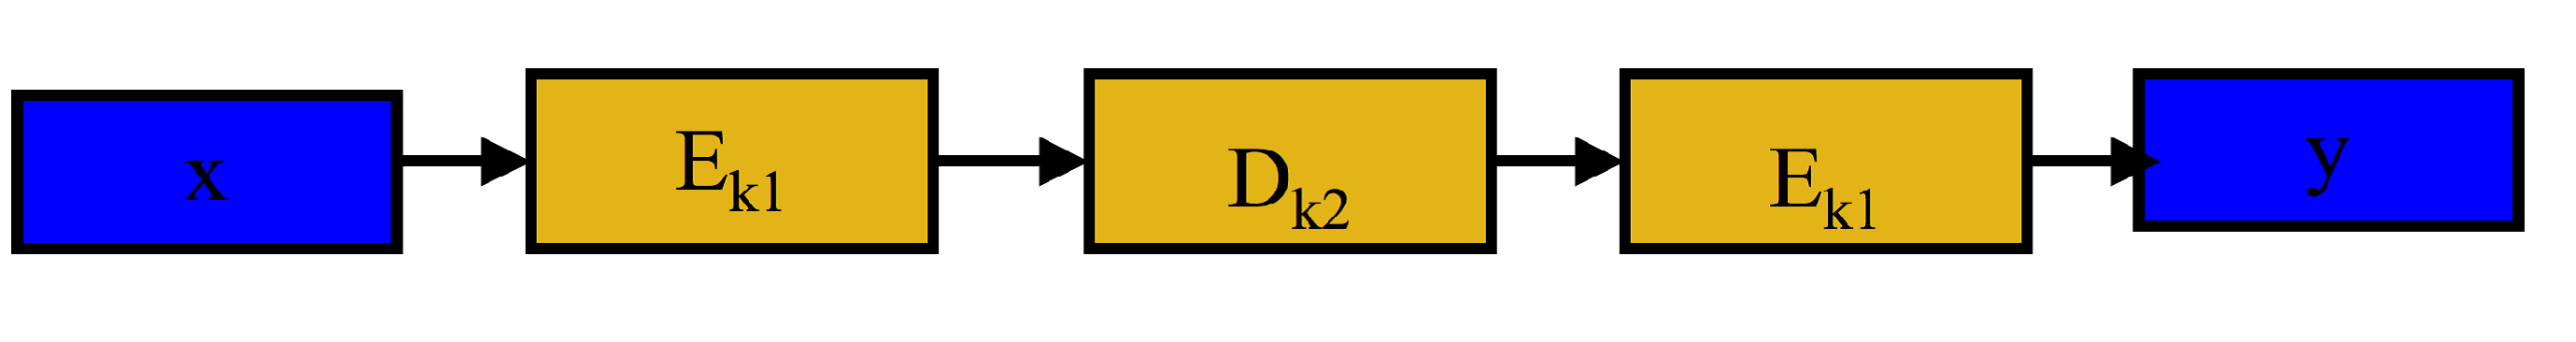
\includegraphics[width=0.5\textwidth]{figures/tcip2}
\par\end{center}
\begin{itemize}
\item The first version utilizes three independent keys $k_{1},k_{2},k_{3}$.
The second, just two - $k_{1},k_{2}$.
\item The \textquotedblplain middle box\textquotedblplain{} employs decryption
rather than encryption. This results in backward compatibility: Taking
$k_{1},k_{2},k_{3}=k$, this is identical to a single encryption using
$k$.
\item When the key is unknown, decryption (should) also be a pseudorandom
function, so using $D_{k_{2}}$ does not reduce security.
\item Both versions are susceptible to a meet in the middle attack, albeit
one that uses a list of size $2^{2n}$ (where $n$ is length of keys).\\
This is the best attack known for version (1).
\item For version (2), there is a $O\left(n2^{n}\right)$ attack using $O\left(2^{n}\right)$
chosen input/output pairs. This substantially reduces the practical
risk of such attack. 
\end{itemize}
\begin{conc}
Security is a subtle issue - Best to have a proof of security.
\end{conc}


\chapter{Authentication}

While encryption focuses on secrecy (privacy), Message Authentication
Codes focus on\textbf{ }\emph{integrity} (ensuring the message wasn't
changed) and \emph{authenticity} (ensuring it really came from Alice).
These goals are \emph{orthogonal}; secrecy alone does not guarantee
integrity.

\section{The Authentication Model}

The goal is to ensure integrity even in the presence of an \emph{active
adversary} (Fran the Forger) who can hear genuine messages, possibly
choose messages to be signed, and then send her own forged messages.
Bob must be able to distinguish genuine messages from forged ones.

\begin{center}
\begin{tikzpicture}[node distance=1.5cm]
    % Defined Colors to match slides
    \definecolor{slideyellow}{RGB}{218,218,0}
    \definecolor{slidegreen}{RGB}{0,180,0}

    % Parties
    \node[person, draw=black, fill=slideyellow] (A) at (0,0) {\textbf{A}};
    \node[person, draw=black, fill=slideyellow, right=5cm of A] (B) {\textbf{B}};
    \node[person, draw=black, fill=slidegreen, dashed] (F) at (2.5,-1.8) {\textbf{F}};
    
    % Labels (Black writing globally)
    \node[below=0.2cm of A, align=center, font=\sffamily\small] {Alice\\(sender)};
    \node[below=0.2cm of B, align=center, font=\sffamily\small] {Bob\\(receiver)};
    \node[below=0.2cm of F, align=center, font=\sffamily\small] {Fran\\(forger)};

    % Communication channel (Alice to Bob)
    \draw[->, >=Stealth, line width=1.5pt] 
        (A.east) -- node[above, pos=0.5, font=\sffamily] {$(m, \tg)$} (B.west);
    
    % Active Adversary Intercept/Forgery
    \draw[<->, >=Stealth, red, dashed, thick] (2.5,-0.1) -- (F.north);

\end{tikzpicture}
\end{center}

In our model, the \textquotedbl major players\textquotedbl{} interact
as follows:
\begin{itemize}
\item \textbf{Parties:} Alice and Bob are the legitimate participants. In
authentication contexts, Alice is the \emph{sender} and Bob is the
\emph{receiver}.
\item \textbf{Adversary:} Fran is the active adversary who tampers with
the message to compromise integrity. 
\item \textbf{Channel: }A reliable communication line exists between Alice
and Bob.
\item \textbf{The Shared Secret:} They utilize an \emph{authentication}
scheme $\mac$ that is \emph{known }to Fran, and a \emph{secret }key
$k$.
\item \textbf{The Goal:} Alice wants to send a message $m$ to Bob such
that it remains untampered with. Bob must be able to tell genuine
messages from forged ones.
\end{itemize}
\begin{mydefinition}[MAC]
 A \textbf{Message Authentication Code} is $\mac:\KK\times\MM\xrightarrow{}\TT$,
$\tg=\mac_{k}\left(m\right)$ is called a \textbf{tag}.
\end{mydefinition}

\section{Security}
\begin{mydefinition}[EU-CPA]
 Consider the following game:

\begin{center}
\begin{tikzpicture}]

    % --- Challenger ---
    \node[chalbox] (C) at (-2.5,0) {
        \textbf{Challenger}\\
        $k \r \KK$\\[6em]
    };

    % --- Adversary ---
    \node[advbox] (A) at (2.5,0) {
        \textbf{Adversary $\mathcal{A}$}\\[7em]
        \textcolor{red}{Output $(m,\tg)$}
    };

	\node at (0,-3em) {$\vdots$};
    % --- Communication ---
    \draw[arrow] ([yshift=3.5em]A.west) -- node[above] {$m_1$} ([yshift=3.5em]C.east);
    \draw[arrow] ([yshift=3em]C.east) -- node[below] {$\mac_k(m_1)$} ([yshift=3em]A.west);
	\draw[arrow] ([yshift=0.25em]A.west) -- node[above] {$m_2$} ([yshift=0.25em]C.east);
    \draw[arrow] ([yshift=-0.25em]C.east) -- node[below] {$\mac_k(m_2)$} ([yshift=-0.25em]A.west);
	
\end{tikzpicture}
\end{center}

The adversary wins if $m\neq m_{i}$ (for all $i$) and $\tg=\mac_{k}\left(m\right)$.
Then MAC has $\left(t,\varepsilon\right)$ \textbf{Existential Unforgeability
under Chosen Plaintext Attack }if for every $t$-bounded adversary
$\mathcal{A}$ which is allowed to ask for $t$ legal pairs, $\Pr\left[\mathcal{A}\text{ wins}\right]\leq\varepsilon$.
\end{mydefinition}
\begin{thm}
If $\mac:\str n\xrightarrow{}\str{\ell}$ is a random function then
it's $\left(\infty,2^{-\ell}\right)$-secure.
\end{thm}
%
\begin{thm}
A $\left(t,\varepsilon\right)$-secure PRF is $\left(t'\approx t,\varepsilon'=\varepsilon+2^{-\ell}\right)$-MAC.
\begin{proof}[Proof idea]
If the PRF was truly random function then hard to forge, hence an
adversary that breaks the MAC can distinguis the PRF from truly random
function.
\end{proof}
\end{thm}

\end{document}
